\documentclass{article}
\usepackage[T1]{fontenc}
\usepackage{lmodern}
\usepackage{graphicx}
\usepackage{amsmath,amssymb}
\usepackage[a4paper,margin=2cm]{geometry}
\usepackage[absolute,overlay]{textpos}
\setlength{\TPHorizModule}{1mm}
\setlength{\TPVertModule}{1mm}
\usepackage[indonesian]{babel}
\usepackage{hyperref}
\setlength{\emergencystretch}{2em}
% unit: Halaman 60

\begin{document}

% === Halaman 60 (llm) ===

\section*{Cipher Berulang (Iterated Cipher)}

\begin{itemize}
    \item Untuk menghasilkan \textit{cipher} yang lebih kuat, maka dilakukan \textit{enciphering} sejumlah kali (sejumlah putaran) .
    \item Caranya adalah dengan melakukan berulang kali suatu fungsi transformasi $f$ (disebut juga fungsi putaran atau \textit{round function}) yang mengubah blok plainteks menjadi blokcipherteks.
    \item Pada setiap putaran digunakan upa-kunci (\textit{subkey}) atau kunci putaran (\textit{round key}) yang dikombinasikan dengan plainteks.
\end{itemize}

\vspace{10mm}

\[ i = 1, 2, ..., n \]

% deskripsi: Diagram blok yang menunjukkan proses iterasi fungsi f dengan loop balik.
% bbox normalisasi: [0.7300, 0.7300, 0.8900, 0.9300]
\begin{textblock*}{33.60mm}(153.30mm,216.81mm)
\noindent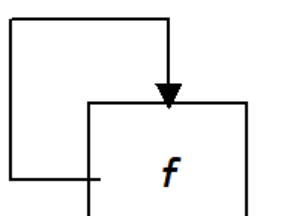
\includegraphics[width=33.60mm,height=59.40mm]{../../images/llm/page_060_img_01.png}%
\end{textblock*}

\end{document}
